
%% bare_conf.tex
%% V1.4b
%% 2015/08/26
%% by Michael Shell
%% See:
%% http://www.michaelshell.org/
%% for current contact information.
%%
%% This is a skeleton file demonstrating the use of IEEEtran.cls
%% (requires IEEEtran.cls version 1.8b or later) with an IEEE
%% conference paper.
%%
%% Support sites:
%% http://www.michaelshell.org/tex/ieeetran/
%% http://www.ctan.org/pkg/ieeetran
%% and
%% http://www.ieee.org/

%%*************************************************************************
%% Legal Notice:
%% This code is offered as-is without any warranty either expressed or
%% implied; without even the implied warranty of MERCHANTABILITY or
%% FITNESS FOR A PARTICULAR PURPOSE! 
%% User assumes all risk.
%% In no event shall the IEEE or any contributor to this code be liable for
%% any damages or losses, including, but not limited to, incidental,
%% consequential, or any other damages, resulting from the use or misuse
%% of any information contained here.
%%
%% All comments are the opinions of their respective authors and are not
%% necessarily endorsed by the IEEE.
%%
%% This work is distributed under the LaTeX Project Public License (LPPL)
%% ( http://www.latex-project.org/ ) version 1.3, and may be freely used,
%% distributed and modified. A copy of the LPPL, version 1.3, is included
%% in the base LaTeX documentation of all distributions of LaTeX released
%% 2003/12/01 or later.
%% Retain all contribution notices and credits.
%% ** Modified files should be clearly indicated as such, including  **
%% ** renaming them and changing author support contact information. **
%%*************************************************************************


% *** Authors should verify (and, if needed, correct) their LaTeX system  ***
% *** with the testflow diagnostic prior to trusting their LaTeX platform ***
% *** with production work. The IEEE's font choices and paper sizes can   ***
% *** trigger bugs that do not appear when using other class files.       ***                          ***
% The testflow support page is at:
% http://www.michaelshell.org/tex/testflow/



\documentclass[conference]{IEEEtran}
% Some Computer Society conferences also require the compsoc mode option,
% but others use the standard conference format.
%
% If IEEEtran.cls has not been installed into the LaTeX system files,
% manually specify the path to it like:
% \documentclass[conference]{../sty/IEEEtran}





% Some very useful LaTeX packages include:
% (uncomment the ones you want to load)


% *** MISC UTILITY PACKAGES ***
%
%\usepackage{ifpdf}
% Heiko Oberdiek's ifpdf.sty is very useful if you need conditional
% compilation based on whether the output is pdf or dvi.
% usage:
% \ifpdf
%   % pdf code
% \else
%   % dvi code
% \fi
% The latest version of ifpdf.sty can be obtained from:
% http://www.ctan.org/pkg/ifpdf
% Also, note that IEEEtran.cls V1.7 and later provides a builtin
% \ifCLASSINFOpdf conditional that works the same way.
% When switching from latex to pdflatex and vice-versa, the compiler may
% have to be run twice to clear warning/error messages.






% *** CITATION PACKAGES ***
%
\usepackage{cite}
% cite.sty was written by Donald Arseneau
% V1.6 and later of IEEEtran pre-defines the format of the cite.sty package
% \cite{} output to follow that of the IEEE. Loading the cite package will
% result in citation numbers being automatically sorted and properly
% "compressed/ranged". e.g., [1], [9], [2], [7], [5], [6] without using
% cite.sty will become [1], [2], [5]--[7], [9] using cite.sty. cite.sty's
% \cite will automatically add leading space, if needed. Use cite.sty's
% noadjust option (cite.sty V3.8 and later) if you want to turn this off
% such as if a citation ever needs to be enclosed in parenthesis.
% cite.sty is already installed on most LaTeX systems. Be sure and use
% version 5.0 (2009-03-20) and later if using hyperref.sty.
% The latest version can be obtained at:
% http://www.ctan.org/pkg/cite
% The documentation is contained in the cite.sty file itself.




% *** GRAPHICS RELATED PACKAGES ***
%
\ifCLASSINFOpdf
  \usepackage[pdftex]{graphicx}
  % declare the path(s) where your graphic files are
  % \graphicspath{{../pdf/}{../jpeg/}}
  % and their extensions so you won't have to specify these with
  % every instance of \includegraphics
  \DeclareGraphicsExtensions{.pdf,.jpeg,.png}
\else
  % or other class option (dvipsone, dvipdf, if not using dvips). graphicx
  % will default to the driver specified in the system graphics.cfg if no
  % driver is specified.
  % \usepackage[dvips]{graphicx}
  % declare the path(s) where your graphic files are
  % \graphicspath{{../eps/}}
  % and their extensions so you won't have to specify these with
  % every instance of \includegraphics
  % \DeclareGraphicsExtensions{.eps}
\fi
% graphicx was written by David Carlisle and Sebastian Rahtz. It is
% required if you want graphics, photos, etc. graphicx.sty is already
% installed on most LaTeX systems. The latest version and documentation
% can be obtained at: 
% http://www.ctan.org/pkg/graphicx
% Another good source of documentation is "Using Imported Graphics in
% LaTeX2e" by Keith Reckdahl which can be found at:
% http://www.ctan.org/pkg/epslatex
%
% latex, and pdflatex in dvi mode, support graphics in encapsulated
% postscript (.eps) format. pdflatex in pdf mode supports graphics
% in .pdf, .jpeg, .png and .mps (metapost) formats. Users should ensure
% that all non-photo figures use a vector format (.eps, .pdf, .mps) and
% not a bitmapped formats (.jpeg, .png). The IEEE frowns on bitmapped formats
% which can result in "jaggedy"/blurry rendering of lines and letters as
% well as large increases in file sizes.
%
% You can find documentation about the pdfTeX application at:
% http://www.tug.org/applications/pdftex





% *** MATH PACKAGES ***
%
%\usepackage{amsmath}
% A popular package from the American Mathematical Society that provides
% many useful and powerful commands for dealing with mathematics.
%
% Note that the amsmath package sets \interdisplaylinepenalty to 10000
% thus preventing page breaks from occurring within multiline equations. Use:
%\interdisplaylinepenalty=2500
% after loading amsmath to restore such page breaks as IEEEtran.cls normally
% does. amsmath.sty is already installed on most LaTeX systems. The latest
% version and documentation can be obtained at:
% http://www.ctan.org/pkg/amsmath





% *** SPECIALIZED LIST PACKAGES ***
%
%\usepackage{algorithmic}
% algorithmic.sty was written by Peter Williams and Rogerio Brito.
% This package provides an algorithmic environment fo describing algorithms.
% You can use the algorithmic environment in-text or within a figure
% environment to provide for a floating algorithm. Do NOT use the algorithm
% floating environment provided by algorithm.sty (by the same authors) or
% algorithm2e.sty (by Christophe Fiorio) as the IEEE does not use dedicated
% algorithm float types and packages that provide these will not provide
% correct IEEE style captions. The latest version and documentation of
% algorithmic.sty can be obtained at:
% http://www.ctan.org/pkg/algorithms
% Also of interest may be the (relatively newer and more customizable)
% algorithmicx.sty package by Szasz Janos:
% http://www.ctan.org/pkg/algorithmicx




% *** ALIGNMENT PACKAGES ***
%
%\usepackage{array}
% Frank Mittelbach's and David Carlisle's array.sty patches and improves
% the standard LaTeX2e array and tabular environments to provide better
% appearance and additional user controls. As the default LaTeX2e table
% generation code is lacking to the point of almost being broken with
% respect to the quality of the end results, all users are strongly
% advised to use an enhanced (at the very least that provided by array.sty)
% set of table tools. array.sty is already installed on most systems. The
% latest version and documentation can be obtained at:
% http://www.ctan.org/pkg/array


% IEEEtran contains the IEEEeqnarray family of commands that can be used to
% generate multiline equations as well as matrices, tables, etc., of high
% quality.




% *** SUBFIGURE PACKAGES ***
%\ifCLASSOPTIONcompsoc
%  \usepackage[caption=false,font=normalsize,labelfont=sf,textfont=sf]{subfig}
%\else
%  \usepackage[caption=false,font=footnotesize]{subfig}
%\fi
% subfig.sty, written by Steven Douglas Cochran, is the modern replacement
% for subfigure.sty, the latter of which is no longer maintained and is
% incompatible with some LaTeX packages including fixltx2e. However,
% subfig.sty requires and automatically loads Axel Sommerfeldt's caption.sty
% which will override IEEEtran.cls' handling of captions and this will result
% in non-IEEE style figure/table captions. To prevent this problem, be sure
% and invoke subfig.sty's "caption=false" package option (available since
% subfig.sty version 1.3, 2005/06/28) as this is will preserve IEEEtran.cls
% handling of captions.
% Note that the Computer Society format requires a larger sans serif font
% than the serif footnote size font used in traditional IEEE formatting
% and thus the need to invoke different subfig.sty package options depending
% on whether compsoc mode has been enabled.
%
% The latest version and documentation of subfig.sty can be obtained at:
% http://www.ctan.org/pkg/subfig




% *** FLOAT PACKAGES ***
%
%\usepackage{fixltx2e}
% fixltx2e, the successor to the earlier fix2col.sty, was written by
% Frank Mittelbach and David Carlisle. This package corrects a few problems
% in the LaTeX2e kernel, the most notable of which is that in current
% LaTeX2e releases, the ordering of single and double column floats is not
% guaranteed to be preserved. Thus, an unpatched LaTeX2e can allow a
% single column figure to be placed prior to an earlier double column
% figure.
% Be aware that LaTeX2e kernels dated 2015 and later have fixltx2e.sty's
% corrections already built into the system in which case a warning will
% be issued if an attempt is made to load fixltx2e.sty as it is no longer
% needed.
% The latest version and documentation can be found at:
% http://www.ctan.org/pkg/fixltx2e


%\usepackage{stfloats}
% stfloats.sty was written by Sigitas Tolusis. This package gives LaTeX2e
% the ability to do double column floats at the bottom of the page as well
% as the top. (e.g., "\begin{figure*}[!b]" is not normally possible in
% LaTeX2e). It also provides a command:
%\fnbelowfloat
% to enable the placement of footnotes below bottom floats (the standard
% LaTeX2e kernel puts them above bottom floats). This is an invasive package
% which rewrites many portions of the LaTeX2e float routines. It may not work
% with other packages that modify the LaTeX2e float routines. The latest
% version and documentation can be obtained at:
% http://www.ctan.org/pkg/stfloats
% Do not use the stfloats baselinefloat ability as the IEEE does not allow
% \baselineskip to stretch. Authors submitting work to the IEEE should note
% that the IEEE rarely uses double column equations and that authors should try
% to avoid such use. Do not be tempted to use the cuted.sty or midfloat.sty
% packages (also by Sigitas Tolusis) as the IEEE does not format its papers in
% such ways.
% Do not attempt to use stfloats with fixltx2e as they are incompatible.
% Instead, use Morten Hogholm'a dblfloatfix which combines the features
% of both fixltx2e and stfloats:
%
% \usepackage{dblfloatfix}
% The latest version can be found at:
% http://www.ctan.org/pkg/dblfloatfix




% *** PDF, URL AND HYPERLINK PACKAGES ***
%
%\usepackage{url}
% url.sty was written by Donald Arseneau. It provides better support for
% handling and breaking URLs. url.sty is already installed on most LaTeX
% systems. The latest version and documentation can be obtained at:
% http://www.ctan.org/pkg/url
% Basically, \url{my_url_here}.




% *** Do not adjust lengths that control margins, column widths, etc. ***
% *** Do not use packages that alter fonts (such as pslatex).         ***
% There should be no need to do such things with IEEEtran.cls V1.6 and later.
% (Unless specifically asked to do so by the journal or conference you plan
% to submit to, of course. )


% correct bad hyphenation here
\hyphenation{op-tical net-works semi-conduc-tor}


\usepackage{subfig}

\begin{document}
%
% paper title
% Titles are generally capitalized except for words such as a, an, and, as,
% at, but, by, for, in, nor, of, on, or, the, to and up, which are usually
% not capitalized unless they are the first or last word of the title.
% Linebreaks \\ can be used within to get better formatting as desired.
% Do not put math or special symbols in the title.
%\title{System Partitioning for 3D ICs:\\Is it even worth it?}
\title{Logic-on-Logic Stacking:\\ Where Should the Clustering Stop?}


% author names and affiliations
% use a multiple column layout for up to three different
% affiliations
\author{\IEEEauthorblockN{Quentin \textsc{Delhaye}}
\IEEEauthorblockA{\'Ecole polytechnique de Bruxelles\\
Universit\'e libre de Bruxelles\\
qudelhaye@ulb.ac.be}
\and
\IEEEauthorblockN{Dragomir \textsc{Milojevic}}
\IEEEauthorblockA{\'Ecole polytechnique de Bruxelles\\
Universit\'e libre de Bruxelles\\
dmilojev@ulb.ac.be}%
}

% conference papers do not typically use \thanks and this command
% is locked out in conference mode. If really needed, such as for
% the acknowledgment of grants, issue a \IEEEoverridecommandlockouts
% after \documentclass

% for over three affiliations, or if they all won't fit within the width
% of the page, use this alternative format:
% 
%\author{\IEEEauthorblockN{Michael Shell\IEEEauthorrefmark{1},
%Homer Simpson\IEEEauthorrefmark{2},
%James Kirk\IEEEauthorrefmark{3}, 
%Montgomery Scott\IEEEauthorrefmark{3} and
%Eldon Tyrell\IEEEauthorrefmark{4}}
%\IEEEauthorblockA{\IEEEauthorrefmark{1}School of Electrical and Computer Engineering\\
%Georgia Institute of Technology,
%Atlanta, Georgia 30332--0250\\ Email: see http://www.michaelshell.org/contact.html}
%\IEEEauthorblockA{\IEEEauthorrefmark{2}Twentieth Century Fox, Springfield, USA\\
%Email: homer@thesimpsons.com}
%\IEEEauthorblockA{\IEEEauthorrefmark{3}Starfleet Academy, San Francisco, California 96678-2391\\
%Telephone: (800) 555--1212, Fax: (888) 555--1212}
%\IEEEauthorblockA{\IEEEauthorrefmark{4}Tyrell Inc., 123 Replicant Street, Los Angeles, California 90210--4321}}




% use for special paper notices
%\IEEEspecialpapernotice{(Invited Paper)}




% make the title area
\maketitle

% As a general rule, do not put math, special symbols or citations
% in the abstract
\begin{abstract}
In this paper, we show evidence that 3D IC stacking is a viable alternative to IC technology scaling.
This is proven by partitioning the system at different clustering grains and highlighting a sweet spot balancing 3D connections and total 3D wire-length.
Using various designs as test cases, we present that around 1000 clusters will allow to cut on average 30\% of the nets and to consider 70\% of the total wire-length in 3D.
\end{abstract}

% no keywords




% For peer review papers, you can put extra information on the cover
% page as needed:
% \ifCLASSOPTIONpeerreview
% \begin{center} \bfseries EDICS Category: 3-BBND \end{center}
% \fi
%
% For peerreview papers, this IEEEtran command inserts a page break and
% creates the second title. It will be ignored for other modes.
\IEEEpeerreviewmaketitle


% An example of a floating figure using the graphicx package.
% Note that \label must occur AFTER (or within) \caption.
% For figures, \caption should occur after the \includegraphics.
% Note that IEEEtran v1.7 and later has special internal code that
% is designed to preserve the operation of \label within \caption
% even when the captionsoff option is in effect. However, because
% of issues like this, it may be the safest practice to put all your
% \label just after \caption rather than within \caption{}.
%
% Reminder: the "draftcls" or "draftclsnofoot", not "draft", class
% option should be used if it is desired that the figures are to be
% displayed while in draft mode.
%
%\begin{figure}[!t]
%\centering
%\includegraphics[width=2.5in]{myfigure}
% where an .eps filename suffix will be assumed under latex, 
% and a .pdf suffix will be assumed for pdflatex; or what has been declared
% via \DeclareGraphicsExtensions.
%\caption{Simulation results for the network.}
%\label{fig_sim}
%\end{figure}

% Note that the IEEE typically puts floats only at the top, even when this
% results in a large percentage of a column being occupied by floats.


% An example of a double column floating figure using two subfigures.
% (The subfig.sty package must be loaded for this to work.)
% The subfigure \label commands are set within each subfloat command,
% and the \label for the overall figure must come after \caption.
% \hfil is used as a separator to get equal spacing.
% Watch out that the combined width of all the subfigures on a 
% line do not exceed the text width or a line break will occur.
%
%\begin{figure*}[!t]
%\centering
%\subfloat[Case I]{\includegraphics[width=2.5in]{box}%
%\label{fig_first_case}}
%\hfil
%\subfloat[Case II]{\includegraphics[width=2.5in]{box}%
%\label{fig_second_case}}
%\caption{Simulation results for the network.}
%\label{fig_sim}
%\end{figure*}
%
% Note that often IEEE papers with subfigures do not employ subfigure
% captions (using the optional argument to \subfloat[]), but instead will
% reference/describe all of them (a), (b), etc., within the main caption.
% Be aware that for subfig.sty to generate the (a), (b), etc., subfigure
% labels, the optional argument to \subfloat must be present. If a
% subcaption is not desired, just leave its contents blank,
% e.g., \subfloat[].


% An example of a floating table. Note that, for IEEE style tables, the
% \caption command should come BEFORE the table and, given that table
% captions serve much like titles, are usually capitalized except for words
% such as a, an, and, as, at, but, by, for, in, nor, of, on, or, the, to
% and up, which are usually not capitalized unless they are the first or
% last word of the caption. Table text will default to \footnotesize as
% the IEEE normally uses this smaller font for tables.
% The \label must come after \caption as always.
%
%\begin{table}[!t]
%% increase table row spacing, adjust to taste
%\renewcommand{\arraystretch}{1.3}
% if using array.sty, it might be a good idea to tweak the value of
% \extrarowheight as needed to properly center the text within the cells
%\caption{An Example of a Table}
%\label{table_example}
%\centering
%% Some packages, such as MDW tools, offer better commands for making tables
%% than the plain LaTeX2e tabular which is used here.
%\begin{tabular}{|c||c|}
%\hline
%One & Two\\
%\hline
%Three & Four\\
%\hline
%\end{tabular}
%\end{table}


% Note that the IEEE does not put floats in the very first column
% - or typically anywhere on the first page for that matter. Also,
% in-text middle ("here") positioning is typically not used, but it
% is allowed and encouraged for Computer Society conferences (but
% not Computer Society journals). Most IEEE journals/conferences use
% top floats exclusively. 
% Note that, LaTeX2e, unlike IEEE journals/conferences, places
% footnotes above bottom floats. This can be corrected via the
% \fnbelowfloat command of the stfloats package.

\section{Introduction}
While CMOS continues to scale, the question of Moore's law sustainability still remains open as we enter the era of 5 and 3nm technologies, already in the pipeline for some ASIC manufacturers\footnote{``3nm transistor has been manufactured TSMC Aims for a \$ 20 Billion Investment for 3nm Chip Production – Looking to Secure Partners Early''}. Many facts could support the previous claim. Here we will cite just a few. 

At device/gate level, gate pitch is not expected to scale further due to photo-lithography limitations. To still allow further area scaling, new type of devices have been proposed (FinFet, nano-wire, etc.) with huge number of device options. These device options impact in a great deal the final Power, Performance, Area (PPA) of a design and thus require careful optimization process during device selection/configuration and standard cell design. Due to the number of options involved, this optimization process, known in the literature as Design-Technology Co-Optimization (DCTO), is becoming more and more complex, requiring a lot of effort.

At logic level, alternative gate architectures have been explored, all aiming to reduce the height of standard cells. While this might look appealing at a first sight (area reduction of a gate with less scaled transistors), this also means that the number of routing tracks per gate decreases. Unfortunately, the number of pins per gate remains constant. After all we need cell inputs and outputs as well as power pins. Reduced cell height will cause overall pin density at the design level to increase, which in turn will cause increased congestion, i.e. design routability problems. To cope with this problem we don't have much choices, we can increase design area and/or improve metal layers used for routing. Both solutions come with a cost penalty. 

Speaking of cost, it is known that advanced CMOS nodes are becoming more and more expensive, mainly because of complex multi-patterning techniques used for circuit manufacturing. Also, manufacturing yields can not reach desired figures, thus limiting the die area and preventing cost-effective manufacturing of big dies used for high-performance computing, network processors, etc. 

To address different issues linked to traditional 2D CMOS scaling, 3D integration technology has been proposed, not as an alternative to CMOS scaling, but as a mean to extend the life-cycle of a given CMOS node. It is known that 3D integration offers benefits over 2D circuits: less wire-length, meaning improved system routability, so less buffer insertion during timing optimization, and therefore less total silicon area (for 1/2 of a footprint), less power and better timing. 

Beyond PPA improvements, 3D stacked circuits also offer the possibility of \emph{technologically heterogeneous circuit} integration. In such circuits, different CMOS processes, each optimized for a given functionality (e.g. high-performance, low-power, memory), can be packaged together with different optimization objectives in mind. 

Today, 3D technology is mature and already widely used for memories (stacked DRAMs), image circuits (smart-phones), high-performance computing (wide IO DRAMs) and re-configurable computing (FPGAs). From the technology perspective, high-density 3D interconnects are readily available (e.g. hybrid bonding) with 3D structure pitch of about 1$\mu$m resulting in very dense die-to-die interconnect. Such 3D technologies allows very fine grain system partitioning. The questions of course is how to design such systems and especially how to decide on the system partitioning, i.e. what functional block should go where. 

In this paper we ... 

%A logic-on-logic 3D IC is a system in which there are several layers of logic stacked.
%The first and most obvious gain of designing such a system is that the gates are closer to each other relatively to a pure 2D IC.
%Bringing the gates together also shorten their interconnections, thus reducing the wire capacitance and IR drop.
%Among the benefit of going 3D, the gain in real estate is not to be neglected.
%Indeed, when a long net is shortened, the hypothetical buffers and repeaters that it needed are no %longer required, freeing some space for the placement tool and decreasing the congestion.
%There are two main concurrent approaches to 3D ICs: monolithic and stacking.

% TODO remove \textit around e.g. and i.e.

\subsection{Previous Work}
As of today there is no full support for 3D integration in commercial EDA tools. Rather, various extensions to existing 2D Place\&Route (P\&R) tools have been proposed in academia and industrial R\&D~\cite{Panth}. % Cite CoolCube?
Extension of such approach with improved 3D, PPA has been proposed in ~\cite{Chang2016}. % Cascade2D
Standard cell clustering problem has also been studied at other step of the design, such as during the P\&R step~\cite{Moura2017}. % ICECS2016 clustering 

All the above mentioned flows relay either on manual system partitioning, or they automate the partitioning decision for the smallest possible functionality, the gate. What remains unclear is what happens in between?  

%Comparison between stacking and M3D: \cite{Samal2017}
\cite{Samal2017} argued that 3D stacking was not practical for fine-grained 3D partitioning due to the size of the TSVs, and that a monolithic integration was the way to go. However, monolithic integration still has couple of issues to solve, such as thermal budget required for sequential FEOL processing. Meanwhile, face-to-face hybrid bonding seams to offer a nice compromise between the amount of 3D interconnect and potential PPA gains.

In this work, we try to understand the grain (i.e. the size of the clusters) at which it would be relevant to consider the architecture.
In particular, we want to show that a very fine grain is not necessary and that a coarser grain --for which their would be no congestion using larger TSVs-- improves as much the performance of the IC.
% Statement: single-cell monolithic 3D does not better than a coarser grain cluster in terms of 3D wire-length.

\section{Problems ans solutions}
\subsection{Optimization objectives}
When partitioning a 2D system into a 3D one, several optimization objectives can be considered, such as: (1) number of 3D nets, (2) total 3D system wire-length, (3) longest 3D net (and/or corresponding critical path), (4) total interconnect power.

Objective (1) is essential since it is driven by the pitch of the 3D connection given by the 3D technology. Obviously we need to match cost-effectiveness of the 3D design and PPA gains. Objective (2) needs to be analyzed to understand overall gains (power, congestion, etc.) while objective (3) focuses on critical path and thus the system performance. With 3D implemented system we hope to reduce the total wire-length by bringing the gates closer to each other. However, the 3D re-routed nets have to pass through the interface between the two gate layers and thus should not be longer than a critical threshold, in order to determine the kind of performance improvement at which we can aim. 
Otherwise, those particularly short nets may become longer when routed in 3D, degrading their performance or even needing additional buffers.

\subsection{Partitioning a Circuit Using a (Hyper)Graph}
Digital integrated circuits are made out of logic gates placed in a 2D plane and connected by wires. Placed circuits can be easily represented with hypergraphs $\mathcal{H}$: let $\mathcal{H} = (V, H)$ be an association between the set of vertices $V$ (\textit{e.g.} the gates, or sets of gates, i.e. gate clusters, or simply clusters) and the set of hyperedges $H$ (\textit{e.g.} the nets). 

Since some of the graph partitioning algorithms cannot be applied to hypergraphs, we sometimes need to transpose a hypergraph into a normal graph using the k-clique model: we keep the same set of vertices, but each hyperedge that contains $k$ vertices becomes a $k$-clique in the new set of edges $E$. This yields a new association $\mathcal{G} = (V, E)$. While such transformations have been criticized (see \cite{IhlerEdmund;WagnerDorothea;Wagner1993}) due to loss of accuracy, this approximation is acceptable for our purpose. % WHY?

When tackling the graph partitioning problem, it can mainly go two ways: minimizing or maximizing the cut, which is given by $\sum_{n \in E_c} w_{n}$, with $w_n$ the weight of the net $n$ in the set of cut edges $E_c$. The corresponding problems are respectively denoted as MIN-CUT and MAX-CUT.

If MIN-CUT seems to make the most sense to be applied on a VLSI circuit for which we aim at limiting the amount of 3D connections, it is not necessarily our case. Indeed, MIN-CUT algorithms such as~\cite{Karypis1999, Aykanat2011, Caldwell2000} are already applied on the design at the floorplan and placement steps of the synthesis flow~\cite{KahngAndrewB.Lienig2011}.

When applying algorithms of the same family on the resulting architecture, we simply find the exact same partitioning as the previous step in the toolchain, yielding few if any new interesting results.

However, if we go the other way and apply a MAX-CUT algorithm on the 2D design, we can highlight interesting correlations between the amount of nets cut and the total 3D wire-length.
Those results will be further presented in section~\ref{sec:res}.

% MIN-CUT: \texttt{hMETIS}~\cite{Karypis1999}.

Goemans and Williamson \cite{Goemans1995} proposed a randomized algorithm for the MAX-CUT problem, guaranteeing that their solution would be at least 0.87856 time the optimal value, using semidefinite programming. Burer et al. \cite{Burer2000} presented an improvement over the SDP relaxation in the form of a rank-two relaxation, and implemented their algorithm in the package \texttt{CirCut}.

On top of using those methods, we want to compute a balanced bi-partitioning of the system, meaning that two partitions of the same size need to be produced, \textit{i.e.} of the same area in our application.

\section{Experimental Setup}
% This is important and should connect to the intro
% and therefore the maximum required 3D pitch, 
To study the impact of the partitioning grain on potential wire-length gains of the 3D design with respect to 2D implementation, we have developed a software tool chain to process placed \& routed designs and partition netlists for 3D integration. 

The tool takes as input a 2D placed \& routed design using \texttt{DEF} file, and geometrical views of standard cells (\texttt{LEF} file) to build usable design data base. Following operations are then performed: (1) Input files are parsed to extract the design; (2) Standard cells are clustered, so that each cluster represents a graph vertex ($V$) where vertex weight represent the total cluster area; (3) Inter-cluster nets are extracted to generate graph edges ($E$) and weight function is calculated for each edge (note that we consider different weights); (4) With that information we can build a hypergraph $H = (E, V)$; (5) This hypergraph can be partitioned using: a) MIN-CUT partitioning (using already available implementations in \texttt{hMETIS}~\cite{Karypis1999} or \texttt{PaToH}~\cite{Aykanat2011})  to minimize, or MAX-CUT (using \texttt{CirCut}) maximize the number of inter-die (or 3D) connections.

\subsection{Clustering}
To generate standard cell clusters we use divisive hierarchical~\cite{Rokach2005} based on the geometry of the design: design is first split vertically into two parts of the same size, then each part is split again, but horizontally.
This process is repeated recursively -- subsequent vertical and horizontal splits -- until the target amount of clusters is reached. In our experiments we consider the cluster sizes from 2 to 32768 in power-of-2 steps. The biggest number of clusters (i.e. the smallest cluster size) has been picked with the gate-count of designs in mind.

\subsection{Designs}
Some details about the designs used in the experiments are given in table~\ref{tab:designs}.
Our design data base uses the following designs: D1) BoomCore: \textit{Berkeley Out-of-Order Machine}, an open source implementation of the RISC-V; D2) MCC: a medium complexity core; D3) \& D4) respectively a core and crossbar sub-circuits of the OpenSparc T2; D5) open source implementation of low-parity density parity check; D6) LDPC 4x4: a highly interconnected implementation of 16 LDPC cores D7) LDPC 4x4 serial: a serial implementation of 16 LDPC cores.

\begin{table}[!t]
% increase table row spacing, adjust to taste
\renewcommand{\arraystretch}{1.3}
\caption{Collection of Designs Used for the Experiments}
\label{tab:designs}
\centering
% Some packages, such as MDW tools, offer better commands for making tables
% than the plain LaTeX2e tabular which is used here.

% sort designs in increaseing order and call them D1

\begin{tabular}{||c|r|r|r||}
\hline
Design & Gates & Nets & Total wire-length\\
\hline
\hline
LDPC & 42471 & 49633 & 242001\\
\hline
BoomCore & 121580 & 137171 & 418217\\
\hline
MCC & 220587 & 234373 & 1047417 \\
\hline
CCX & 185777 & 200999 & 5698294\\
\hline
SPC & 289812 & 306118 & 10479466\\
\hline
LDPC 4x4 Serial & 694082 & 773679 & 6023683\\
\hline
LDPC 4x4 & 808199 & 883295 & 10872106\\
\hline
\end{tabular}
\end{table}

\section{Results}\label{sec:res}




% \begin{figure*}
%   \centering
%   \subfloat{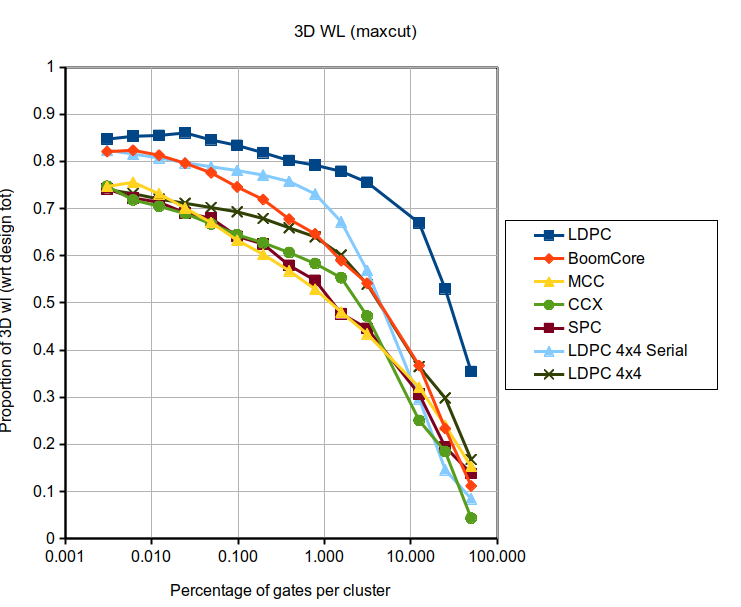
\includegraphics[scale=0.25]{prop-3Dwl-wrt-design_prop-gate-per-clusters_maxcut_v4.png} 
%   \hfill
%   \subfloat{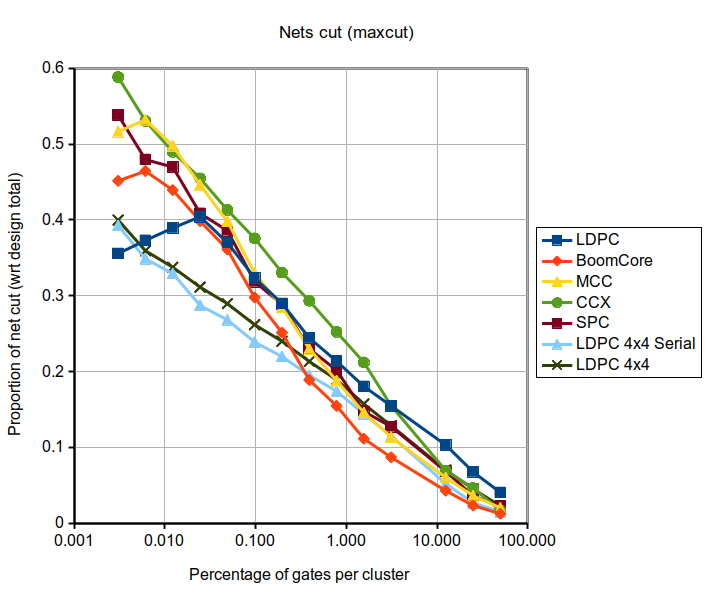
\includegraphics[scale=0.25]{prop-netcut-wrt-design_prop-gate-per-clusters_maxcutv3.png} 
%   \caption{a) The total 3D wire-length increases when the amount of gate per cluster decreases, until it reaches a threshold and b) The total of net cut by the partitioning increases when the amount of gate per cluster decreases, \textit{i.e.} when the amount of clusters increases.}
%   \label{fig:3Dwl}
% \end{figure*} 


% \begin{figure}[!t]
% \centering
% 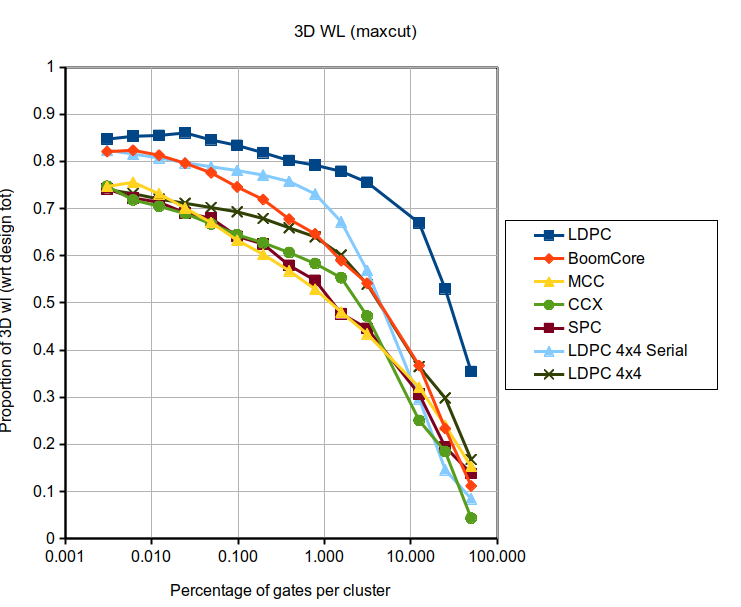
\includegraphics[width=\linewidth]{prop-3Dwl-wrt-design_prop-gate-per-clusters_maxcut_v4.png}
% \caption{The total 3D wire-length increases when the amount of gate per cluster decreases, until it reaches a threshold.}
% \label{fig:3Dwl}
% \end{figure}

% \begin{figure}[!t]
% \centering
% 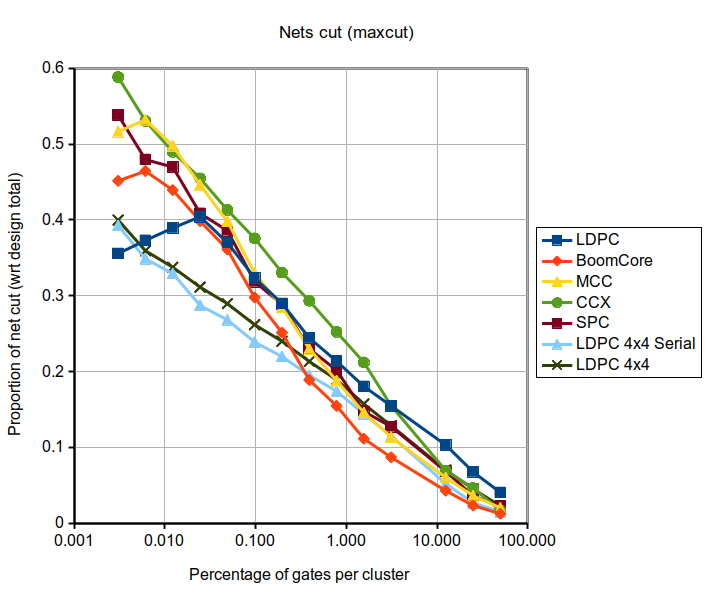
\includegraphics[width=\linewidth]{prop-netcut-wrt-design_prop-gate-per-clusters_maxcutv3.png}
% \caption{The total of net cut by the partitioning increases when the amount of gate per cluster decreases, \textit{i.e.} when the amount of clusters increases.}
% \label{fig:3Dnets}
% \end{figure}

After partitioning the systems, a post-processing script analyzes all the cut nets to determine their quantity and wire-length.
The results are summarized in figures \ref{fig:3Dwl} and \ref{fig:3Dnets}.
In both cases, the measures are given for each level of clustering as a proportion of gates per cluster, \textit{e.g.} for 100 clusters, each cluster hosts on average 1\% of all the gates in the design.
Since all the clusters have the same size and the distribution of gates after the placement step is roughly homogeneous, it seems fair to admit that all clusters host the same amount of gates.
Consequentially an increase of clusters quantity, a finer clustering grain and a decrease of gates per cluster all have the same meaning.

Figure~\ref{fig:3Dwl} shows the proportion of 3D wire-length with respect to the total length of the design.
We clearly see two stages: a first exponential growth of 3D wire-length when there are few clusters, and a second linear growth leading to a plateau.

Figure~\ref{fig:3Dnets} shows the proportion of nets cut by the partitioning with respect to the total amount of nets in the design.
Except occasional hiccups, the growth is exponential all through the finest clustering grain.

In order to limit the 3D pitch, it is important to cut as few wires as possible.
On the other hand, one of the aim of going 3D is to reduce the length of those wire, hence we try to have as much 3D wire-length as possible.

As the amount of wires cut keeps increasing with the number of clusters, the focus needs to be steered toward the total 3D wire-length.
The later reaching a threshold, it becomes ideal to define a sweet spot when the 3D wire-length spots increasing, or at the very least when its increase rate decreases.

Such sweet spot can be set around the 0.1\% of gates per cluster mark.
This value corresponds to 1024 clusters and means that by cutting from 24\% to 38\% of all nets, we can reduce up to 63\% to 83\% of the total wire-length, depending on the considered design (see table~\ref{tab:res}).

\begin{table}[!t]
% increase table row spacing, adjust to taste
\renewcommand{\arraystretch}{1.3}
\caption{MAX-CUT Results for Three Cluster Sizes}
\label{tab:res}
\centering
% Some packages, such as MDW tools, offer better commands for making tables
% than the plain LaTeX2e tabular which is used here.
\begin{tabular}{||c||r|r|r||r|r|r||}
\cline{2-7}
\multicolumn{1}{c||}{} & \multicolumn{3}{c||}{Percentage of nets cut} & \multicolumn{3}{c||}{Percentage of 3D WL}\\
\cline{2-7}
\multicolumn{1}{c||}{} & 2 & 1024 & 32768 & 2 & 1024 & 32768\\
\cline{2-7}
\hline
LDPC & 4\% & 32\% & 36\% & 35\% & 83\% & 85\%\\
\hline
BoomCore & 1\% & 30\% & 45\% & 11\% & 75\% & 82\%\\
\hline
MCC & 2\% & 33\% & 52\% & 15\% & 63\% & 75\%\\
\hline
CCX & 2\% & 38\% & 59\% & 4\% & 64\% & 75\%\\
\hline
SPC & 2\% & 32\% & 54\% & 14\% & 64\% & 74\%\\
\hline
LDPC 4x4 & 2\% & 26\% & 40\% & 17\% & 69\% & 74\%\\
\hline
LDPC 4x4 serial & 1\% & 24\% & 39\% & 8\% & 78\% & 82\%\\
\hline
\end{tabular}
\end{table}

%\begin{figure}[!t]
%\centering
%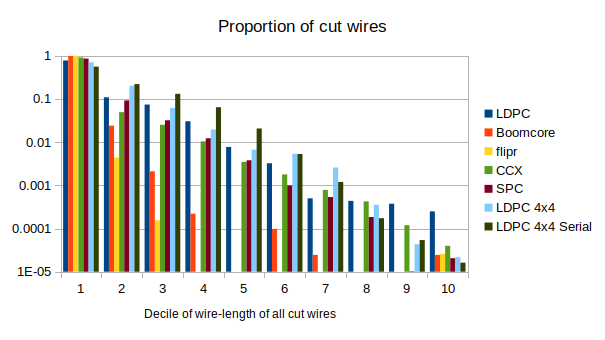
\includegraphics[width=\linewidth]{netCutWL_maxcut_all.png}
%\caption{Distribution of the nets cut by the partition, according to the decile of wire-length to which the net belongs.}
%\label{fig:dist-cut-wires}
%\end{figure}

%Figure~\ref{fig:dist-cut-wires} shows the length of the cut wires.
%The data has been split into deciles according to the length of the length of all the cut wires.
%It is interesting to note that the vast majority of wires belongs to the first decile, \textit{i.e.} are among the shortest in the design.



\begin{figure}[!t]
\centering
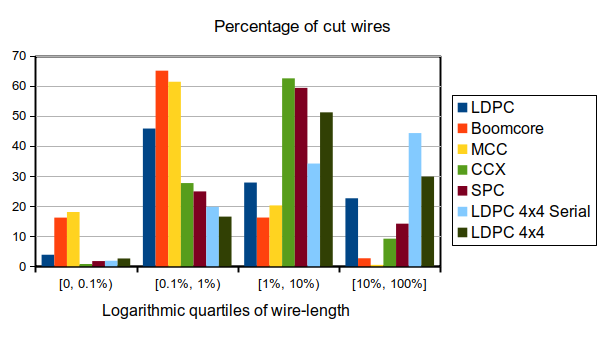
\includegraphics[width=\linewidth]{netCutWL_maxcut_all_log-quartv3.png}
\caption{Distribution of the percentage of cut wires per logarithmic quartile of their wire-length relative to the longest net, for 1024 clusters.}
\label{fig:dits-wl-quart}
\end{figure}

Figure~\ref{fig:dits-wl-quart} show that for most designs, the nets cut by the partition have a length between 0.1\% to 10\% of the longest net cut.
In particular, it highlights the fact that the shortest nets are a minority, hence limiting the drop of performance when rerouting those in 3D.



\section{Conclusion}
In this paper, we showed that there exist a sweet spot for the clustering grain, which balances the amount 3D nets and the total 3D wire-length.
The existence of this equilibrium tells us that we do not need to consider the circuit at a very fine grain; that a coarse grain is adequate.
Hence the 3D stacking is still a viable option and we do not need to bother with a monolithic integration.

In our future work, we could explore other clustering methods in order to further reduce the amount of short net in the partitioning cut.



% conference papers do not normally have an appendix


% use section* for acknowledgment
% \section*{Acknowledgment}






% trigger a \newpage just before the given reference
% number - used to balance the columns on the last page
% adjust value as needed - may need to be readjusted if
% the document is modified later
%\IEEEtriggeratref{3}
% The "triggered" command can be changed if desired:
%\IEEEtriggercmd{\enlargethispage{-5in}}

% references section

% can use a bibliography generated by BibTeX as a .bbl file
% BibTeX documentation can be easily obtained at:
% http://mirror.ctan.org/biblio/bibtex/contrib/doc/
% The IEEEtran BibTeX style support page is at:
% http://www.michaelshell.org/tex/ieeetran/bibtex/
\bibliographystyle{IEEEtran}
% argument is your BibTeX string definitions and bibliography database(s)
\bibliography{bibliography}
%
% <OR> manually copy in the resultant .bbl file
% set second argument of \begin to the number of references
% (used to reserve space for the reference number labels box)
%\nocite{*}



% that's all folks
\end{document}
